\section{if-conversion的运行机制}

控制依赖的概念最早由Ferrante等人提出\cite{ferrante1987prodepgraitsuseopt},RK算法由Park跟Schlansker提出\cite{JosephC.H.Park1991},Hyperblock的概念由Mahlke等人给出\cite{ScottA.Mahlke1992a},逆向if-conversion则是Warter等人的研究成果\cite{Warter1993}。

\subsection{控制依赖}

\begin{definition}[控制流图(control flow graph)]
控制流图是一个有向图,它有唯一的入口节点START以及唯一的出口节点STOP,图中每一个节点最多有两个后继。对于那些有两个后继的节点,它的两条出边分别被赋予属性T(真)跟F(假)。对于图中的每个节点N,都存在从START到N,以及从N到STOP的路径。
\end{definition}

\begin{definition}[后控制(post-dominate)]
设V与W是控制流图G中的节点,如果从V到STOP的每条路径(起始位置的V并不计算在路径中)都包含W,则称V被W后控制,或者W后控制V,记为$W \pdom V$。
\end{definition}

\begin{definition}[直接后控制(immediate post-dominate)]
设X,Y以及Z是控制流图G中的节点,如果$Y\pdom X$,并且对于任意的满足$Z\pdom X$以及$Z\neq Y$的节点Z,都有$Z\pdom Y$,则称Y直接后控制X,或者X被Y直接后控制,记为$Y \ipdom X$
\end{definition}

\begin{definition}[pdom函数]
设N是节点的集合,pdom是一个映射,它将N中的节点x映射为所有后控制x的节点的集合,即$pdom: N\to 2^N$。pdom的定义的数学表述为:$pdom\left(x\right):=\left\{y\in N: y \pdom x\right\}$
\end{definition}

\begin{definition}[ipdom函数]
设N是节点的集合,ipdom是一个映射,它将N中的节点x映射为x直接后控制的节点的节点,即$pdom: N\to N$。ipdom的定义的数学表述为:$ipdom\left(x\right):=y\in N,\text{其中}y \ipdom x$
\end{definition}

\begin{definition}[后控制节点树]
直接后控制关系构成一个树,称为后控制节点树。树的节点为控制流图G中的节点,若$y\ipdom x$,则y是x的双亲节点。显然,求$ipdom\left(x\right)$即为求x在树中的双亲节点,求$pdom\left(x\right)$即为求x在树中的所有祖先节点的集合。
\end{definition}
计算图G的后控制节点树的算法见\fref{app:algo_ipdom_tree}

\begin{definition}[控制依赖(control dependent)]
设G为控制流图,X以及Y是图中节点,称Y控制依赖于X当且仅当:
\begin{enumerate}
\item 存在从X到Y的路径P,使得Y后控制P上除了X与Y的所有节点。
\item X不被Y后控制
\end{enumerate}
\end{definition}
从定义可以看出,如果Y控制依赖与X,则那么X必然有两个出口,其中一条出口导致Y必然被执行,另一条出口则导致Y可能不被执行。

\begin{definition}[CD函数]
设N是节点的集合,C是控制依赖的集合。CD函数是一个映射,它将N中的节点x映射为x的所有控制依赖的集合,即$CD:N\to 2^C$。若将C中的元素$c\in C$表示为$\pm y$,其中$+y$表示y的true边,$-y$表示y的false边,则CD函数的定义可以为:$CD\left(x\right):=\left\{\pm y:x\text{控制依赖于}\pm y\right\}$
\end{definition}
CD函数的计算算法如\fref{alg:ComputeCD}

\begin{algorithm}[H]
	\label{alg:ComputeCD}
	\caption{ComputeCD}
	\KwIn{G是控制流图,N是G中节点的集合,E是G中边的集合}
	\KwOut{CD函数}
	计算函数$pdom\left(x\right)$以及$ipdom\left(x\right)$\;
	\For{每个$\left[x,y,label\right]\in E$并且$y\notin pdom\left(x\right)$}{
		Lub = ipdom(x)\;
		\If{$\neg label$}{$x= -x$\;}
		$t=y$\;
		\While{$t\neq Lub$}{
			$CD\left(t\right)=CD\left(t\right)\cup\left\{x\right\}$\;
			$t=ipdom\left(t\right)$\;
		}
	}
\end{algorithm}

\subsection{RK算法}

CD函数并非是一个单值函数,不同的x可能对应相同的$CD\left(x\right)$。由于具有相同控制依赖的不同节点的执行条件相同,所以将节点转化为谓词执行以后,他们的谓词也应该相同,这样就可以为CD函数的值域中的每个元素分配一个与之一一对应的谓词p,谓词跟值域中元素的集合的对应关系记为K函数。显然,K函数是个单值函数,它的逆$K^{-1}$必然存在,记函数$R=CD\cdot K^{-1}$。可以看出,这么做将CD函数分解为R函数跟K函数:$CD=R\cdot K$。其中R函数负责将每个节点x与谓词p对应起来,而K则将每个谓词跟其对应的控制依赖对应起来。通过R函数,具有相同控制依赖(因而具有相同执行条件)的不同节点被映射到同一个谓词,也就是说,R函数为每个节点实现的谓词分配,节点x对应的谓词$p=R\left(x\right)$。至于K函数,则将每个谓词跟其控制依赖对应起来,这也为谓词的定义提供了参考。一种不错的谓词定义策略是,对于每一个谓词,在其对应的依赖,的相应节点末尾插入相应的赋值语句。例如$K\left(p\right)=\left\{y,-z\right\}$,则在y与z节点插入p的定义语句。插入的时候,如果对该点依赖值为正,则谓词的值就是分支条件,如果为赋,作为谓词的值就是该点分支条件的非。例如上面例子中,在y点插入$p=t_y$,而在z点插入$p=\neg t_z$。R函数以及K函数的计算算法如\fref{alg:ComputeRK}所示。

\begin{algorithm}[H]
	\label{alg:ComputeRK}
	\caption{ComputeRK}
	\KwIn{CD是控制依赖函数,N是G中节点的集合}
	\KwOut{R函数以及K函数}
	p = 1\tcc*{谓词命名从1开始顺序命名}
	\For{$x\in N$}{
		$t = CD\left(x\right)$\;
		\eIf{$t\in K$}{
			$R\left(x\right)=q$,其中q为使得$K\left(q\right)=t$的谓词\;
		}{
			$K\left(p\right)=t$\;
			$R\left(x\right)=p++$\;
		}
	}
\end{algorithm}
计算好R函数以及K函数,并按照R函数跟K函数进行谓词分配与定义以后,只要对控制流图进行拓扑排序即可得到转换后的代码。if-conversion的算法如\fref{alg:ifcvt}。

\begin{algorithm}[H]
	\label{alg:ifcvt}
	\caption{If-Conversion}
	\KwIn{G是控制流图,N是G中节点的集合,E是G中边的集合}
	\KwOut{转换后的代码}
	计算CD函数\;
	计算RK函数\;
	\For{$x\in N$}{
		$p=R\left(x\right)$\;
		\If{$K\left(p\right)\neq\varnothing$}{
			给x分配谓词$p$\;
		}
	}
	\For{每个谓词p}{
		\For{$\pm y\in K\left(p\right)$}{
			若是$+y$则在y尾部插入$p=t_y$\;
			若是$-y$则在y尾部插入$p=\neg t_y$;
		}
	}
	对G进行拓扑排序,删掉分支语句,并对已分配谓词的基本块进行谓词化\;
\end{algorithm}

%例如,如下控制流图:
%举个例子说明一下

\subsection{Hyperblock}

\begin{definition}[Hyperblock]
Hyperblock是一个谓词化的基本块的集合,这个集合只有一个入口,但是可以有多个出口。
\end{definition}

哪些基本块被包含在Hyperblock中,哪些不被包含在Hyperblock中,这个的选择比较自由,可以根据需要选择,比如说把不经常被执行的基本块,或者太过长的基本块排除在外,而把经常执行又短小精悍的基本块包含在内。
自由选择的基本块不一定满足Hyperblock的定义,比如\fref{fig:taildup}以及\fref{fig:looppeeling}的(a),这时候就需要对控制流图进行一定的处理,这样才能使选择的基本块能够构成一个Hyperblock。

对不满足定义的基本块的集合处理的一种变换是\textbf{尾复制(Tail Duplication)},另一种是\textbf{循环剥离(loop peeling)}。尾复制过程如\fref{fig:taildup}所示,图中(a)是分支选择的结果,(b)是尾复制以后的结果,(c)是if-conversion之后的结果。
\begin{figure}
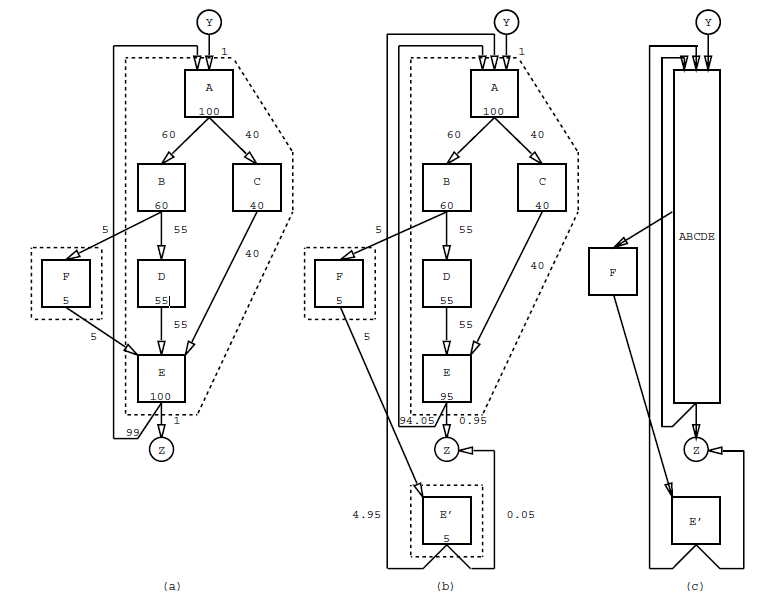
\includegraphics[width=\linewidth]{hyperblock-td}
\caption{\label{fig:taildup} 尾复制}
\end{figure}

循环剥离的过程如图\fref{fig:looppeeling}所示,图中(a)是分支选择的结果,(b)是循环剥离以后的结果。
\begin{figure}
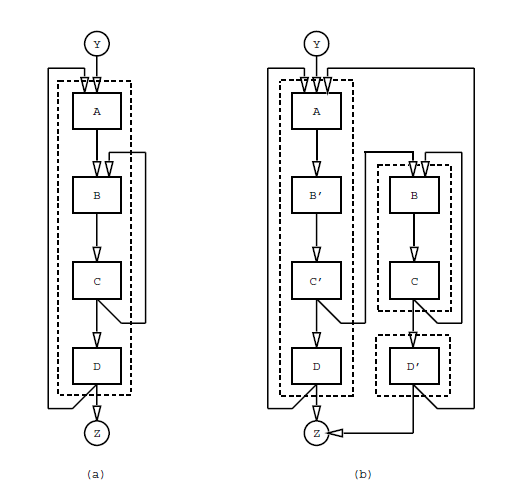
\includegraphics[width=\linewidth]{hyperblock-lp}
\caption{\label{fig:looppeeling} 循环剥离}
\end{figure}

\subsection{逆向if-conversion}

逆向if-conversion能够将谓词化的语句重新转换成分支语句,其算法如下:
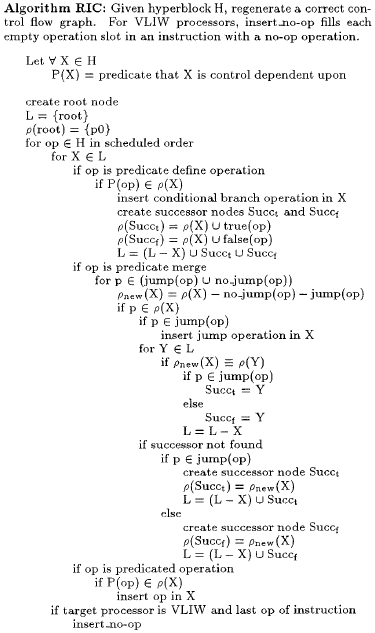
\includegraphics[width=\linewidth]{RIC}